\documentclass[a4paper,ngerman,12pt]{scrartcl}

\usepackage[utf8]{inputenc}
%\usepackage[ansinew]{inputenc}

\usepackage[ngerman]{babel}

\usepackage{amsmath,amsthm,amssymb,stmaryrd,color,graphicx}
\usepackage{setspace}
\usepackage{bussproofs}
\usepackage{array}
\usepackage{comment}
\usepackage{wrapfig}

\usepackage{enumitem}

\usepackage{units}

\usepackage[protrusion=true,expansion=true]{microtype}

\usepackage{lmodern}

\usepackage{hyperref}
\usepackage{cleveref}

\newcommand{\RR}{\mathbb{R}}
\newcommand{\CC}{\mathbb{C}}
\newcommand{\ZZ}{\mathbb{Z}}
\newcommand{\NN}{\mathbb{N}}
\newcommand{\QQ}{\mathbb{Q}}

\setlength\parskip{\medskipamount}
\setlength\parindent{0pt}

\theoremstyle{definition}
\newtheorem{defn}{Definition}[]
\newtheorem{axiom}[defn]{Axiom}
\newtheorem{bsp}[defn]{Beispiel}

\theoremstyle{plain}
\newtheorem{prop}[defn]{Proposition}
\newtheorem{motto}[defn]{Motto}
\newtheorem{wunder}[defn]{Wunder}
\newtheorem{ueberlegung}[defn]{Überlegung}
\newtheorem{lemma}[defn]{Lemma}
\newtheorem{kor}[defn]{Korollar}
\newtheorem{hilfsaussage}[defn]{Hilfsaussage}
\newtheorem{satz}[defn]{Satz}
\newtheorem{frage}[defn]{Frage}

\theoremstyle{remark}
\newtheorem{bem}[defn]{Bemerkung}
\newtheorem{aufg}[defn]{Aufgabe}

\newtheorem*{antwort}{Antwort}

\newlength{\aufgabenskip}
\setlength{\aufgabenskip}{1.4em}
\newcounter{aufgabennummer}
\newenvironment{aufgabe}[1]{
	\addtocounter{aufgabennummer}{1}
	\textbf{Aufgabe \theaufgabennummer.} \emph{#1} \par
}{\vspace{\aufgabenskip}}

\clubpenalty=10000
\widowpenalty=10000
\displaywidowpenalty=10000

\setlength\unitlength{1cm}

\usepackage{tikz}

\RequirePackage{geometry}
\geometry{textwidth=16.0cm,textheight=24.5cm,footskip=1.5cm}

\usepackage{todonotes}


\begin{document}
	
\begin{picture}(0,0)
\put(0,-0.5){%
	
\includegraphics[scale=0.1]{logo-ifm}
}
\put(14.0,-3.5){%
	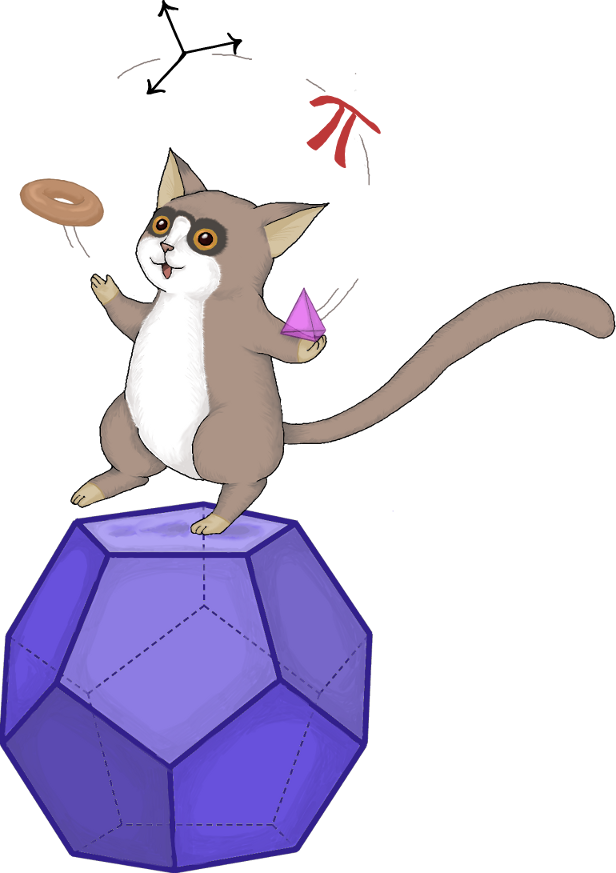
\includegraphics[scale=0.17]{cover}
}
\end{picture} 
	
\vspace{6em}

\begin{center}\Large{Vierter Korrespondenzbrief}\end{center}

\section*{Erste Beweise mit Induktion}

In diesem Brief werden wir eine besondere, in der Mathematik sehr oft genutzte Beweistechnik kennen lernen: Den \emph{Beweis durch Induktion}. Eine Besonderheit dieser Beweistechnik ist, dass man mit ihr nicht nur eine Aussage, sondern gleich unendlich viele Aussagen auf einmal zeigen kann! 

\section{Induktion mit Bildern}

Vor kurzem habe ich mal wieder mein  Sparschein geleert um es zur Bank zu bringen. Davor wollte ich aber natürlich wissen, wie viel Geld sich überhaupt darin befunden hatte. Und um mir das Zählen zu erleichtern (und vielleicht auch, weil mir gerade ein wenig langweilig war) habe ich die Münzen zu einem Muster zusammengelegt:

\begin{center}
	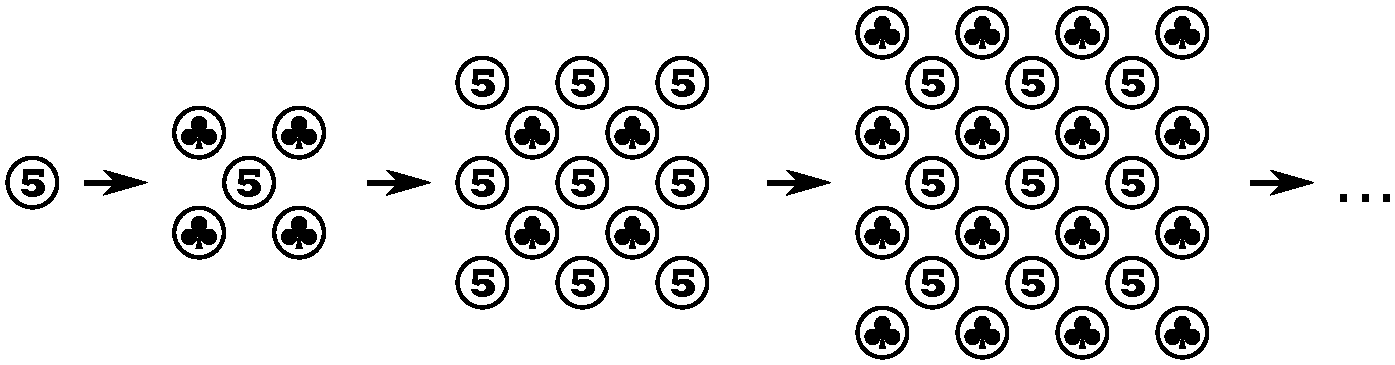
\includegraphics[width=.6\textwidth]{bilder/ZentrierteViereckszahlen.pdf}
\end{center}

\begin{aufgabe}{Der nächste Schritt}
	Erkennst du das Schema, nach dem ich dieses Muster gebaut habe? Kannst du das nächste Viereck zeichnen?
\end{aufgabe}

Während ich also immer größere Vierecke gelegt habe, ist mir das folgende aufgefallen: Die Zahl an Münzen, die ich für ein Viereck benötige, scheint immer eine ungerade Zahl zu sein: Für das erste $1$, beim zweiten $5$, beim dritten $13$, beim vierten $25$, beim fünften \underline{\phantom{ 41 }}(?), \dots

Ob das wohl für alle solchen Vierecke stimmt? Ich habe noch ein paar weitere solchen Vierecke gelegt, und für tatsächlich habe ich für jedes eine ungerade Anzahl an Münzen gebraucht. Aber irgendwann sind mir natürlich die Münzen ausgegangen. Wie kann ich nun also herausfinden, ob meine Vermutung wirklich für \emph{alle} solche Vierecke gilt?

Wir haben nun also für ein paar kleine Beispiele gesehen, dass die Aussage \glqq Für ein (zentriertes) Viereck benötigt man eine ungerade Zahl an Münzen.\grqq{} für diese stimmt. Wir können nun aber nicht \emph{alle} möglichen Vierecke durchprobieren und für jedes einzelne prüfen, ob die Aussage auch für diese stimmt.

Ein ähnliches Problem hatten wir zu Beginn dieses Schuljahres schon einmal in einem Zirkelbrief? Erinnerst du dich noch an den Brief mit den Unmöglichkeitsbeweisen? Den Tetrominos, den Schachbrettern und den Chamäleons? 

\begin{center}
	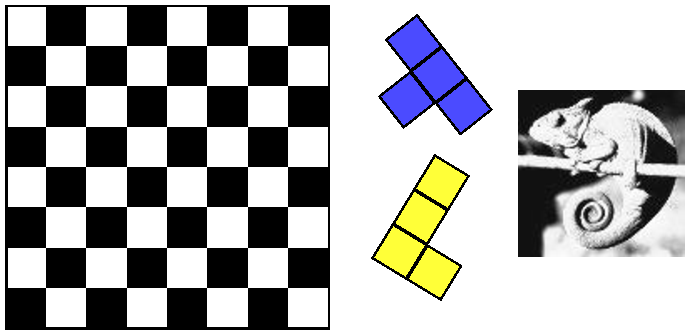
\includegraphics[width=.25\textwidth]{bilder/Erinnerung.pdf}
\end{center}

Darin hatten wir doch ein ganz ähnliches Problem: Wir hatten zum Beispiel eine Menge verschiedenfarbiger Chamäleons, die ihre Farbe nach einem bestimmten Muster ändern, wenn sie sich treffen. Wir wollten nun zeigen, dass wir nie gleich viele Chamäleons jeder Farbe bekommen können.

Dazu haben wir den Begriff einer \emph{Invariante} eingeführt: Eine Aussage, die ganz am Anfang wahr ist und die bei jedem Zwischenschritt (Treffen zweier Chamäleons) erhalten bleibt. Letzteres heißt: Vorausgesetzt die Invariante gilt vor dem Treffen zweier Chamäleons, dann gilt sie auch nach dem Treffen wieder. Dadurch wussten wir dann, dass diese Aussage zu jedem Zeitpunkt gilt - und wir konnten daraus folgern, dass es nie gleich viele Chamäleons jeder Farbe geben wird.

Ganz ähnlich wollen wir nun auch mit unseren Münzvierecken vorgehen, um zu zeigen, dass wir immer eine ungerade Anzahl von Münzen benötigen:

\begin{description}
	\item[Anfang:] Für das kleinstmögliche Viereck (mit Seitenlänge $1$) ist die Aussage klar: Es besteht aus genau einer Münze - und $1$ ist eine ungerade Zahl.
	\item[Voraussetzung:] Wir haben ein Viereck mit Seitenlänge $n$, für das wir bereits wissen, dass wir für es ungerade viele Münzen benötigen.
	\item[Schlussfolgerung:] Wir wollen nun zeigen, dass auch ein Viereck mit Seitenlänge $n+1$ ungerade viele Münzen benötigt. Dazu nehmen wir unser Viereck mit Seitenlänge $n$ und machen daraus ein Viereck der Seitenlänge $n+1$:
	\begin{center}
		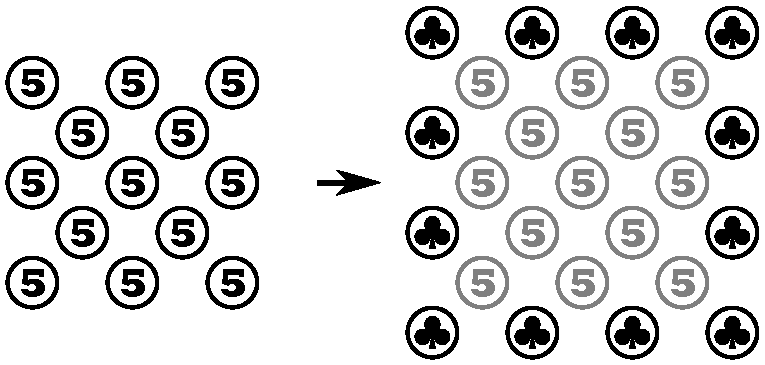
\includegraphics[width=.4\textwidth]{bilder/ZentrierteViereckszahlenBeweis.pdf}
	\end{center}
	Was müssen wir dazu also machen? Wir fügen auf jeder Seite zusätzlich eine Reihe Münzen hinzu $(\ast)$. Da wir nun auf jeder der vier Seiten gleich viele Münzen hinzufügen, ist die Zahl der neuen Münzen sicher durch $4$ teilbar, also eine gerade Zahl.
	
	Die Gesamtzahl der Münzen im $(n+1)$-Viereck ist also gleich der Zahl der Münzen im $n$-ten Viereck (ungerade!) plus der Zahl der neuen Münzen (gerade!). Da nun die Summe einer geraden und einer ungeraden Zahl wieder eine ungerade bildet
	\footnote{Du bist skeptisch, ob diese Aussage wirklich für alle Zahlen gilt? Sehr gut! In der Mathematik sollte man nie irgendwelche Behauptungen einfach so glauben, sondern sie am besten selbst nachprüfen. Teste die Aussage am besten mal an ein paar Beispielen. Wenn du sie wirklich beweisen willst, dann schau dir noch einmal den zweiten Korrespondenzbrief (zu Teilbarkeit) an - darin findest du alle dafür notwendigen Werkzeuge.},
	ist also auch die Zahl der Münzen in unserem größeren Viereck erneut eine ungerade Zahl.
\end{description}

Damit haben wir nun bewiesen, dass alle nach dem beschriebenen Schema gelegten Vierecke eine ungerade Anzahl von Münzen benötigen. Warum?

Nun, wenn wir ein Viereck mit irgendeiner beliebigen Seitenlänge (z.B. $n$) bauen wollen, dann können wir zunächst mal mit dem kleinstmöglichen Viereck beginnen (dem mit Seitenlänge $1$). Dafür benötigen wir eine ungerade Zahl an Münzen (nämlich eine) - das haben wir im Abschnitt \glqq Anfang\grqq{} gezeigt.

Dieses Viereck können wir nun schrittweise immer größer machen (erst zu einem mit Seitenlänge $2$, dann zu einem mit Seitenlänge $3$ usw.), bis wir bei der gewünschten Größe angekommen sind. Und wie wir oben gezeigt haben, kommt in jedem Schritt eine gerade Anzahl von Münzen hinzu. Hatten wir also vor einem Schritt eine ungerade Zahl Münzen verwendet (\glqq Voraussetzung\grqq ), so haben wir auch nach diesem Schritt insgesamt eine ungerade Anzahl Münzen benutzt (\glqq Schlussfolgerung\grqq ).

Insbesondere wissen wir damit, dass wir auch am Ende - wenn wir die gewünschte Größe erreicht haben - insgesamt eine ungerade Zahl Münzen verbaut haben.

\begin{aufgabe}{Wie viele neue Münzen?}
	Im obigen Beweis wird an der Stelle $(\ast)$ nur gesagt, dass die Zahl der neuen Münzen durch $4$ teilbar ist. Kannst du sogar herausfinden, wie viele Münzen es genau sind (in Abhängigkeit von $n$)?
	
	Anders gesagt: Wie viele zusätzliche Münzen benötigt man, um aus einen Viereck mit Seitenlänge $n$ eines mit Seitenlänge $n+1$ zu machen?
\end{aufgabe}

\begin{aufgabe}{Zentrierte Dreieckszahl}
	Natürlich kann man aus Münzen nicht nur Vierecke legen, sondern zum Beispiel auch Dreiecke:
	\begin{center}
		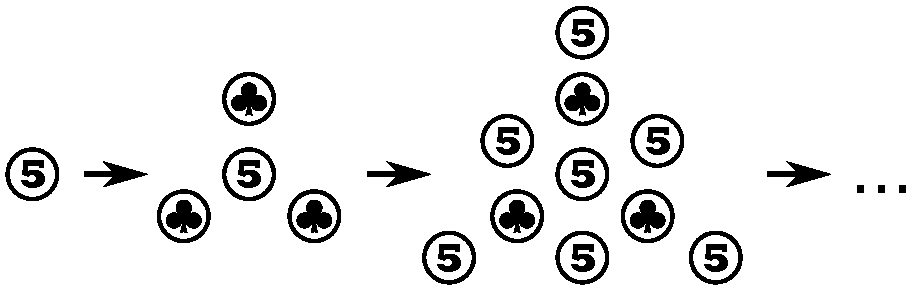
\includegraphics[width=.4\textwidth]{bilder/ZentrierteDreieckszahlen.pdf}
	\end{center}	
	Zeige, dass die zentrierte Dreieckszahl nie durch $3$ teilbar ist (du kannst sogar noch genauer zeigen, dass sie immer um $1$ größer ist als eine durch $3$ teilbare Zahl).
\end{aufgabe}


\section{Induktion mit Zahlen}

Die Beweistechnik, die wir im vorangegangen Abschnitt kennengelernt haben, bezeichnet man als \emph{Beweis durch Induktion} oder \emph{Induktionsbeweis}. Bevor wir nun weitere Beispiele für solche Beweise kennenlernen, wann wir Induktion verwenden können und \todo{bessere Formulierung!}aus welchen Bausteinen sie besteht:

Mittels Induktion kann man Aussagen über \glqq Objekte\grqq{} beweisen, die folgende Eigenschaft haben: Es gibt unter ihnen ein oder mehrere \glqq kleinste\grqq{} Objekte und alle anderen Objekte können wir aus diesen kleinsten durch einen oder mehrere Zwischenschritte erhalten.

Ein Induktionsbeweis besteht dann aus folgenden drei Komponenten:

\begin{description}
	\item[Induktionsanfang (IA):] Wir beweisen die Aussage für das oder die kleinsten Objekte von Hand.
	\item[Induktionsvoraussetzung (IV):] \todo{weiter}
	\item[Induktionsschluss (IS):] Wir beweisen, dass die Aussage durch die Zwischenschritte erhalten bleibt: \todo{weiter}
\end{description}


Einen natürlichen Kandidaten für Induktionsbeweise bildet nun die Menge der natürlichen Zahlen ($\mathbb{N} = \{1,2,3, \dots\}$). Denn diese hat ein kleinstes Objekt ($1$) und alle anderen ihrer Elemente kann man aus diesem durch einen oder mehrere Zwischenschritte erhalten (nämlich ein- oder mehrmals $+1$ rechnen).
\footnote{Tatsächlich werden die natürlichen Zahlen in der Mathematik oft genau durch diese Eigenschaft definiert - nämlich über die \emph{Peano-Axiome}.}

Wann immer man also auf eine Aussage der Form \glqq Für alle natürlichen Zahlen $n \in \NN$ gilt \dots\grqq{} trifft, lohnt es sich auszuprobieren, ob man hier mit Induktion weiter kommt!

\begin{satz}\label{satz:zentrierteViereckszahl}
	Für alle natürlichen Zahlen $n$ gilt: $2n^2-2n+1$ ist eine ungerade Zahl.
\end{satz}

\begin{proof}
	Wir werden diese Aussage mittels Induktion zeigen:
	\begin{description}
		\item[IA ($n=1$):] $2n^2-2n+1  = 2\cdot 1^2 -2 \cdot 1 + 1 = 2-2+1 = 1$ ist ungerade.
		\item[IV (festes $n$):] Für festes $n$ sei $2n^2-2n+1$ eine ungerade Zahl.
		\item[IS ($n \to n+1$):] Wir wollen die Aussage für die Zahl $n+1$ zeigen unter der Voraussetzung, dass die Aussage für die nächstkleinere Zahl (also $n$) bereits gezeigt wurde:
		\[2(n+1)^2-2(n+1)+1  = 2n^2+4n+2-2n-2+1 = (2n^2-2n+1) + 4n\]
		ist ungerade, da $2n^2-2n+1$ nach IV ungerade ist und $4n$ gerade ist. \qedhere
	\end{description}
\end{proof}

\begin{aufgabe}{Durch $3$ teilbar?}\label{aufg:zentrierteDreieckszahl}
	Zeige mittels Induktion die folgende Behauptung:
	
	Für jede natürliche Zahl $n$ ist die Zahl \todo{welche Zahl?} durch $3$ teilbar.
\end{aufgabe}

\begin{aufgabe}{De-ja-vu\todo{Rechtschreibung prüfen!}}\label{aufg:dejavu}
	Berechne $2n^2-2n+1$ für $n = 1,2,3,4,5$. Fällt dir etwas auf? (Schau am besten nochmal in den ersten Abschnitt!) 
	
	Kannst du deine Vermutung sogar beweisen? Evtl. geht das mit einem Induktionsbeweis, der einen Großteil der Struktur des Beweises von \Cref{satz:zentrierteViereckszahl} übernimmt.
	
	Zusatzfrage: Findest du einen ähnlichen Zusammenhang für die Zahl aus Aufgabe \ref{aufg:zentrierteDreieckszahl}?
\end{aufgabe}

\begin{aufgabe}{Induktion oder Nicht-Induktion?}
	Beweise: Für jede natürliche Zahl $n$ ist $2n^2-2n+1$ die Summe zweier direkt aufeinander folgender Quadratzahlen.
	
	Diese Aufgabe kannst du mit Induktion, aber auch direkt (durch Termumformung) zeigen. Wenn du Aufgabe \ref{aufg:dejavu} gelöst hast, kannst du die Behauptung hier sogar durch ein Bild zeigen!
\end{aufgabe}


\section{Anwendungen der Induktion}

\subsection{Geometrisches}

Im letzten Korrespondenzbrief (zu Fraktalen) haben wir unter anderem die \emph{Kochsche Schneeflocke} betrachtet:
\begin{center}
	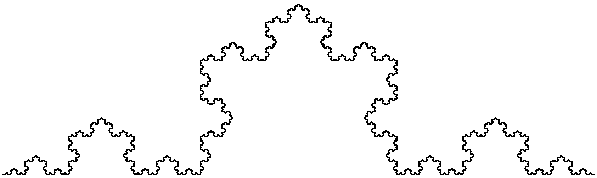
\includegraphics[width=.4\textwidth]{bilder/Schneeflocke-Konstruktion3.pdf}
\end{center}
Nur noch mal zur Erinnerung, wie man die Kochsche Schneeflocke (bzw. erstmal nur eine ihrer drei Seiten) erhält: Man beginnt mit einer einfachen Strecke. Diese Strecke teilt man in drei gleich lange Teile. Dann entfernt man das mittlere Stück und ersetzt es durch die zwei anderen Seiten eines gleichseitigen Dreiecks. Dadurch erhält man eine geometrische Figur, die aus vier Strecken besteht. Für den zweiten Schritt macht man nun mit jeder dieser vier Strecken das gleiche wie man es mit der ersten Strecke getan hat:
\begin{center}
	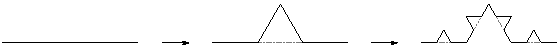
\includegraphics[width=.9\textwidth]{bilder/Schneeflocke-Konstruktion1.pdf}
\end{center}
Und das geometrische Objekt, das man \glqq nach unendlich vielen Schritten\grqq{} erhält, das nennt man dann Kochschee Schneeflocke.

Im letzten Korrespondenzbrief habe ich behauptet, dass die Länge der Linie, aus der die Kochsche Schneeflocke besteht \emph{unendlich} lang ist. Der Beweis dazu war aber noch etwas ungenau: Wir haben nur gesehen, dass die Linie in den ersten beiden Schritten um jeweils mindestens \unit[1]{cm} wächst - und dann einfach behauptet, dass das \glqq offensichtlich\grqq{} auch für alle weiteren Schritte so sein wird.

Jetzt aber haben wir die Technik des Induktionsbeweises kennen gelernt - und diese eignet sich perfekt um genau solche Argumente mathematisch präzise zu machen. 

\begin{satz}
	Beginnt man die Konstruktion einer Seite der Kochschen Schneeflocke mit einer Linie der Länge \unit[3]{cm}, so ist die Linie nach dem $n$-ten Schritt mindestens \unit[3+n]{cm} lang.
\end{satz}

Bevor du weiter liest: Kannst du dir so ungefähr vorstellen, wie der Induktionsbeweis für diese Aussage aussehen könnte? Was wird wohl der Induktionsanfang sein, was die Induktionsvoraussetzung und was der Induktionsschluss?

\begin{proof}
	Wir beweisen den Satz durch Induktion über $n$:
	\begin{description}
		\item[IA ($n=1$):] Nach dem ersten Schritt besteht die Linie aus $4$ Strecken, die jeweils einem Drittel der Anfangsstrecke entsprechen, also jeweils \unit[1]{cm} lang sind. Die Gesamtlänge der Linie beträgt daher $4 \cdot \unit[1]{cm} = \unit[4]{cm} = \unit[3+1]{cm}$.
		\item[IV:] Wir wissen für festes $n$: Nach dem $n$-ten Schritt hat die Linie die Länge \unit[x]{cm}, wobei gilt $x \geq 3+n$.
		\item[IS ($n\to n+1$):] Im $(n+1)$-ten Schritt machen wir mit jeder Teilstrecke das gleiche, was wir im ersten Schritt mit der Anfangsstrecke gemacht haben. Dadurch wird also jede Strecke durch ein Linienstück ersetzt, das $\frac{4}{3}$-mal so lang ist. Dabei wird natürlich auch die Gesamtlinie um den Faktor $\frac{4}{3}$ gestreckt. Nach dem Schritt gilt also für die Gesamtlänge:
			\begin{align*}
			\text{Länge } 	&= \frac{4}{3}\cdot \unit[x]{cm} \overset{\text{\textbf{IV}}}{\geq} \frac{4}{3}\cdot \unit[(3+n)]{cm} = \unit[(4+\frac{4}{3}\cdot n)]{cm} > \unit[(4+ n)]{cm} \\
							&= \unit[(3+ (n+1))]{cm}
			\end{align*}
		Und das ist genau das, was wir zeigen wollten!
	\end{description}
\end{proof}

\begin{aufgabe}{Ein flächenloses Dreieck}
	\todo[inline]{Analog: Die Fläche des Sierpinski-Dreiecks ist $0$}
\end{aufgabe}

\todo[inline]{Beweise über Bäume? Evtl. als "echte" Bäume beschreiben und nur kurzer Hinweis auf Graphentheorie? Evtl. als Lückenbeweis}

\subsection{Ein Abzählspiel}

\todo[inline]{Einleitung: Stell dir vor du triffst dich mit einigen Freunden ...}

\todo[inline]{Ein Beispiel durchrechnen (mit Bildern!) Für $n$=8?}

\begin{frage}
	Verwendet eine Gruppe von $n$ Personen das oben beschriebene Abzählverfahren, welche Person bleibt dann am Ende übrig.\todo{Recherchieren!}
	\footnote{Diese Fragestellung ist auch als Josephus-Problem bekannt, da das ihr zugrunde liegende Abzählverfahren erstmals vom jüdischen Geschichtsschreiber Josephus beschrieben wird.}
\end{frage}

\begin{aufgabe}{Einige Beispiele}
	Spiele das Verfahren einmal für verschiedene (kleine) Gruppengrößen durch und beobachte jeweils, welche Person am Ende übrig bleibt. Fülle dazu die folgende Tabelle:
	\begin{center}
		\renewcommand{\arraystretch}{2}
		\begin{tabular}{l||c|c|c|c|c|c|c|c|c}
			Gruppengröße:	& 2	& 3 & 4 & 5 & 6 & 7 & 8 & 11 & 16 \\\hline
			Letzte Person:	&   &   &   &   &   &   & 0 &    &    
		\end{tabular}
	\end{center}
	Kannst du irgendein Muster erkennen? 
\end{aufgabe}

\todo[inline]{Weiter}

% Alternativer/Zusätzlich möglicher letzter Abschnitt: Korrektheitsbeweise
%Induktion verwendet man auch für Korrektheitsbeweise von Computerprogrammen:
%
%Beispiel: Quadratzahl $x^2$ berechnen als $x+x-1 +x-1+x-2 + \dots +1$ - evtl. dargestellt als Flussdiagramm (rekursives Programm!)
%
%Aufgabe?
%
%Euklidischer Algorithmus? Verweis auf zweiten Brief

\end{document}